%
% latex-sample.tex
%
% This LaTeX source file provides a template for a typical research paper.
%

%
% Use the standard article template.
%
\documentclass[12pt]{article}

% The geometry package allows for easy page formatting.
\usepackage{geometry}

% Load up special logo commands.
\usepackage{doc}

% Package for formatting URLs.
\usepackage{hyperref}

% Packages and definitions for graphics files.
\usepackage{graphicx}
\usepackage{epstopdf}
\usepackage{setspace}

% To generate dummy text
\usepackage{lipsum}

% To adjust title location
\usepackage{titling}

\usepackage{amsmath}
\usepackage{amssymb}
\usepackage[utf8]{inputenc}
\usepackage{url}
\usepackage{listings}

%\doublespacing
\onehalfspacing
%\setlength{\droptitle}{5em}   % This is your set screw

\makeatletter    
\def\@maketitle{
	\centering
	
%	{\Huge \bfseries \sffamily \@title }\\[4ex] 
	{\LARGE \@title }\\ [60mm]
	
\includegraphics[width = 40mm]{boun} \\[5mm]
	{\large \@author}\\[5mm] 
	\@date\\

}
\makeatother

% set up graphics path
\graphicspath{{./img/}}

\newcommand{\myitem}{\refstepcounter{enumi}\item[$*$\theenumi.]}

%\DeclareGraphicsRule{.tif}{png}{.png}{`convert #1 `dirname #1`/`basename #1 .tif`.png}

%
% Set the title, author, and date.
%

%\tit1{Cmpe 492  Final Project \\[10mm] Midterm Report }
%\tit2{A Matchmaking \& Ranking System\\ via \\ Bayesian Inference}
\title{Cmpe 492  Final Project \\[1mm] Midterm Report \\[60mm] Player Rating \& Matchmaking\\ via \\[3mm] Bayesian Inference}
	 

\author{Mustafa Onur Eken\\ advised by A. Taylan Cemgil}
\date{2016}

%
% The document proper.
%

\geometry{
	a4paper,
	total={170mm,257mm},
	left=30mm,
	top=25mm,
	right=30mm,
	bottom=30mm,
}
\begin{document}

% Add the title section.
\maketitle
\thispagestyle{empty}
\newpage
% Add an abstract.
%\abstract{}

% Add various lists on new pages.
\pagebreak
\tableofcontents

\pagebreak




%\listoffigures
%\pagebreak
%\listoftables
% Start the paper on a new page.
%\pagebreak

%
% Body text.
%
\section{Introduction \& Motivation}

We can safely say that player rating systems are essential nearly to any game in different contexts (video games, sports etc). This need arises from the fact that an \textit{unbalanced} match is not enjoyable to any of it's competitors. In an \textit{unbalanced}  match, there is a high variation among the skills of the competitors, therefore a remarkable challenge is not achieved and inadequate amount of fun is generated.

Assuming the fact that the skill levels of the players in a match is the dominant factor affecting the result of that match, if we could figure out skill levels of players of a particular game then we could arrange \textit{balanced} matches that are entertaining for both highly and poorly skilled players. 

With this motivation, Arpad Elo developed a rating system for the board game Chess \cite{wiki:elo}. According to his mathematical modeling, rating of a player is a unit-less positive number. System has an expected result for a match between two players and when the actual result is observed the ratings of the players are updated. Winner's rating always goes up and loser's rating goes down but unexpected (\textit{upsetting}) results magnify the amount of change in the ratings.

In this project we are going to study and implement a generalized and improved version of Elo rating system, developed by Microsoft Research , \textit{TrueSkill}. It is generalized because matches are not constrained as to be one versus one and unlike Elo, \textit{TrueSkill }learns more from the stalemates. In addition, it converges on players' ratings faster.

From a rating system three major functionalities are expected: 1) Estimating skills 2) Suggesting \textit{balanced} matches and 3) Publishing skills
\section{State of the Art}

Currently, many commercial online multi-player video games use Elo rating system where the system is slightly modified  according to specific needs of the game. A rating system called Glicko, newer than Elo older than TrueSkill, is also used in some video games such as \textit{Counter Strike: Global Offensive} \cite{wiki:glicko}. TrueSkill extends ideas presented in Glicko rating system and it is  deployed on \textit{Xbox Live}.

\newpage
\section{Methods}
\subsection{Theory}
TrueSkill can be considered a Bayesian model-based machine learning algorithm \cite{bishop2013model, herbrich2006trueskill}. It assumes a graphical model for a match \cite{alpaydin2014ml} and executes an algorithm on the graph (model) to infer better estimates about the skills of player involved in the match. We will go into details in the subsequent paragraphs.

The model can be described in plain text as following:

\begin{enumerate}

	\item \textbf{Player Model}
	\begin{itemize}
		\item We denote \textit{estimated} skill of the player $i$ as $\mu_i$
		\item System is uncertain about skills of players. The uncertainty associated with a skill, $\mu_i$, of a player is $\sigma_i$
		\item System thinks the \textit{actual }skill of the player, $s_i$, is normally distributed with parameters $\mu_i$ and $\sigma^2_i$		
		\item A player can generate a performance, $p_i$, depending on his/her actual skill, $s_i$. $p_i$ is normally distributed with mean $s_i$ and with variance $\beta^2$, where $\beta$ is a constant depending on chance factor associated with that particular type of game. For instance, one can expect $\beta$ chosen for \textit{Uno} to be larger than $\beta$ chosen for \textit{Chess}. See \cite{moser} for details.
	\end{itemize}

	\item \textbf{Team Model}
	\begin{itemize}
		\item Teams are formed by players and can contain any number of players
		\item Similar to the player model, a team can generate a performance, $t_i$. It is simply obtained by summing up the performances of member players, $\sum p_i$, so $t_i$ is normally distributed as well.
%		\item When comparing two teams and estimating the winner, the system uses \textit{performances} of teams, $t_i$
%		\item For a team, the team performance, $t_i$, is obtained by simply summing up performances of individual players in that team, $\sum p_i$
	\end{itemize}

	\item \textbf{Match Model}
	\begin{itemize}
		\item Instead of players, only teams compete in a match. 
		\item A match result is a relative standings of teams involved in that match. Different teams may have same rank in the standings which indicates a draw. The top team in the standings is the winner.
		\item In a match, teams' performances are compared, i.e. subtracted from each other, $d_i$ (\textit{team performance difference}). With these $d_i$ system expects some teams rank higher than others and vice versa.
	\end{itemize}	
\end{enumerate}
And finally, for the system to infer new $\mu_i$ and $\sigma_i$ (recall that this is our essential desire: to find better estimates for players' skills) the actual result of the match is compared with the expected outcomes, i.e. $d_i$. In a multi-team match, we are going to compare only the teams that are neighbors in the standings (\textit{i.e. in the actual results}) of the match. See Figure \ref{factorgraph} for a visual representation of the model of an example match where three teams and four players are involved. 

\begin{figure}
	\centering
	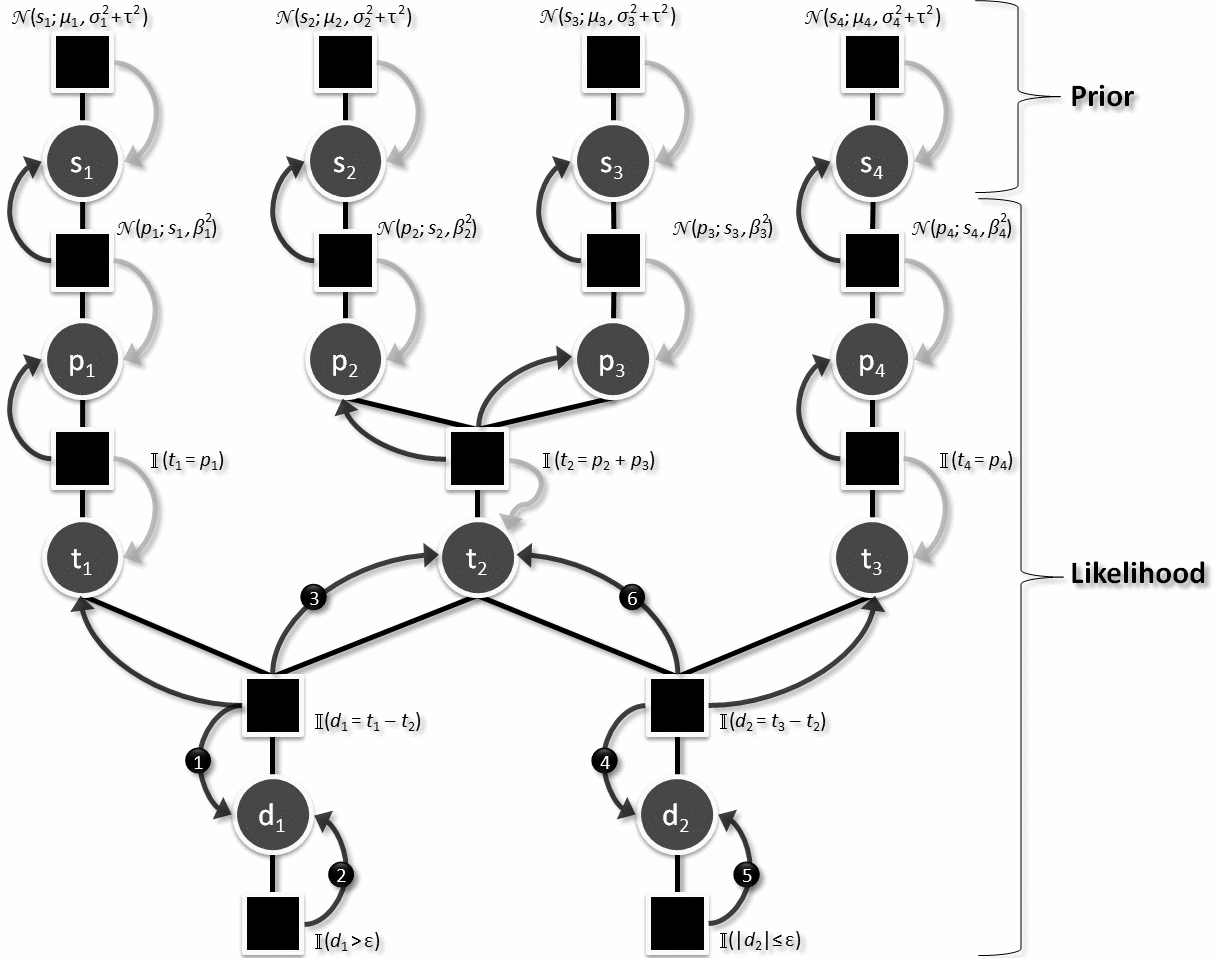
\includegraphics[width=0.6\columnwidth]{factorgraph}
	\caption{A factor graph for a particular match}
	\label{factorgraph}
\end{figure}
A factor graph represents the factorization of a function of several variables \cite{loeliger2001factor}. The functions (a.k.a. \textit{functor nodes}) are drawn as square blocks in the example factor graph shown in Figure \ref{factorgraph}. Most functions can be read and interpreted easily from the Figure \ref{factorgraph} such as $\mathcal{N}(p_1;s_1,\beta_1 ^2)$ but some cannot, e.g. $\mathbb{I}(d_1 > \epsilon)$. See \cite{herbrich2006trueskill} for details of those functions. The whole graph together forms a joint distribution over all variables, in example above it is  $f(s_1,s_2,s_3,s_4,p_1,p_2,p_3,p_4,t_1,t_2,t_3,d_1,d_2)$. We are only interested in marginal distributions of actual skill variables: $f(s_1)$, $f(s_2)$, $f(s_3)$, $f(s_4)$. Note that, we expect these distributions to be Gaussian with new expected skill, $\mu^{new}_i$, and new uncertainty $\sigma^{new}_i$ parameters, refer to \cite{herbrich2006trueskill} for the reasoning. Knowing these, we can use sum-product message passing  algorithm \cite{loeliger2001factor} to solve for the marginal distributions in the factor graphs that we create for each match.

\subsection{Implementation}
After we comprehend the theory and math behind the graphical model and belief propagation algorithm described, implementation comes next. We have chosen \textit{Python 2.7.11} as the language and \textit{Sphinx} for documenting the project. The following are the steps we decided to follow in the implementation period:
\begin{enumerate}
	\singlespacing	
	\itemsep 0em
	\myitem Setup documentation system
	\myitem \textit{Model} module: implement \textit{Player, Team, Match, Environment} classes
	\myitem Implement synthetic data generation
	\myitem \textit{FactorGraph} module: implement \textit{FactorNone, VariableNode, FactorGraph} classes
	\myitem Implement factor graph generation based on a match object
	\item Implement sum-product message passing algorithm
	\item Test on synthetic data and fix bugs
	\item Implement match quality measurer
	\item Test on synthetic data and fix bugs
	\item Implement skill publishing
	\item Test on synthetic data and fix bugs
	\item Implement match recommender
	\item Test on synthetic data and fix bugs
	\item Fetch and format real world data, example dataset: tennis matches \cite{tennis}
	\item Test on real world data	
	\item Finalize documentation and prepare demonstrations
\end{enumerate}
The steps with $*$ are completed, see the git repository \url{https://github.com/oeken/reelskill}. Currently we have the backbone classes and we can generate dummy data with a call of a function. By using a particular seed number for our random number generators we ease the debugging. For now, data generator generates a specified number of players, a specified number of teams each sized equally and all matches that could take place between two teams from the team list. I.e. $T \choose 2$ matches where $T$ is the number of the teams.

\textit{FactorGraph} class is implemented in a doubly linked list manner to ease implementation of future steps such as sum-product algorithm. After generating some data, we can generate the full factor graph for a match object. Graph generator works recursively, for a match it creates sub-graphs for each team and connects the leaf nodes of the sub-graphs. Similarly for a team it creates sub-graphs for each player and connects the leaf nodes of the sub-graphs.

Next we are going to implement the most important part of TrueSkill, \textit{the sum-product algorithm}. After completion of this, we achieve the the first and the most important function of our rating system: 1) Estimating skills. The remaining functionalities are relatively straightforward to implement. Furthermore, we possess a good real world data in our hands: tennis matches. Since it is well organized, we can test TrueSkill on it as soon as the implementation of belief propagation algorithm finishes.

\section{Results}
This section will be available in the final report.
\section{Conclusion \& Discussion}
This section will be available in the final report.
\section{Future Work}
This section will be available in the final report.

% Generate the bibliography.
\bibliography{refs}
\bibliographystyle{unsrt}

\end{document}
